\documentclass[11pt, oneside]{article}
\usepackage{geometry}
\geometry{letterpaper}
\usepackage{graphicx}
\usepackage{amssymb}
\usepackage{amsmath}
\usepackage{tikz}
\usepackage{tikz-qtree}
\usepackage{url}
\usepackage[T1]{fontenc}

\title{SICP Exercise 3.14}
\author{Yuchong Pan}

\begin{document}
\maketitle

In general, \url{mystery} reverses a given list. The box-and-pointer diagram that represents the list to which \url{v} is bound is given as follows.

\begin{figure}[h!]
    \centering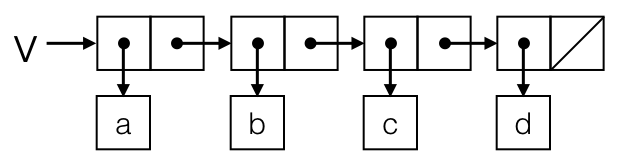
\includegraphics[width=7.5cm]{ex-3.14-1.png}
    \caption{Effect of \textbf{(define v (list 'a 'b 'c 'd))}.}
\end{figure}

After evaluating \textbf{(define w (mystery v))}, the box-and-pointer diagrams that show the structure \url{v} and \url{w} are given as follows.

\begin{figure}[h!]
    \centering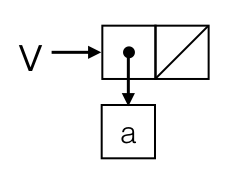
\includegraphics[width=2.5cm]{ex-3.14-2.png}
    \caption{Structure of \textbf{v} after evaluating \textbf{(define w (mystery v))}.}
\end{figure}

\begin{figure}[h!]
    \centering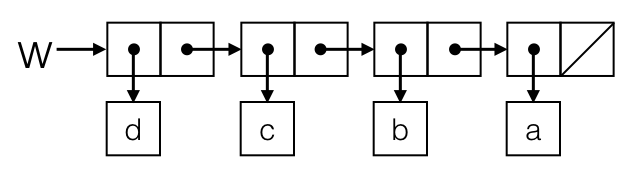
\includegraphics[width=7.5cm]{ex-3.14-3.png}
    \caption{Structure of \textbf{w} after evaluating \textbf{(define w (mystery v))}.}
\end{figure}

\textbf{(a)}, \textbf{(d c b a)} would be printed as the values of \url{v} and \url{w}, respectively.

\end{document}
